\documentclass[11pt,usenames,dvipsnames,aspectration=169]{beamer}
%\usetheme{cern}
\usetheme{cernomc}

% Beamer Setup ---
\setbeamercovered{transparent=5} 
\setbeamertemplate{navigation symbols}{} 

\AtBeginSection{%
	\begin{frame}[noframenumbering]{Outline}
	\tableofcontents[currentsection]
	\end{frame}
}

% Imports ---
\usepackage[utf8]{inputenc}
\usepackage{amsmath}
\usepackage{amsfonts}
\usepackage{amssymb}
\usepackage{mathtools}
\usepackage{bm}  % bold math
\usepackage{xcolor}  % define colors
\usepackage{graphicx}
\usepackage{grffile}  % filenames with dots 
\usepackage{tikz}
\usepackage{hyperref}
\usepackage{siunitx}
\usepackage{booktabs}
\usepackage{multirow}
\usepackage{caption}
\usepackage[absolute,overlay]{textpos}

\graphicspath{{./images}{./images/beamtest}}
\newcommand{\highl}[1]{\textbf{#1}}


% Meta ------------------------------------------------------------------------
\author[OMC]{Andreas Wegscheider on behalf of the OMC team}
\title[LHC 2022]{LHC Commissionning 2022}
\logo{} 
\institute{CERN}
\date[09.06.22]{09.06.2022}
\subject{} 

% Document ---------------------------------------------------------------------
\begin{document}

% \frontcover  % just the cern frontcover, wouldn't use it


\begin{frame}
    \titlepage
\end{frame}


\begin{frame}{Full Outline}
\tableofcontents
\end{frame}
\small

\section{Injection Optics}
\begin{frame}{Injection optics}
    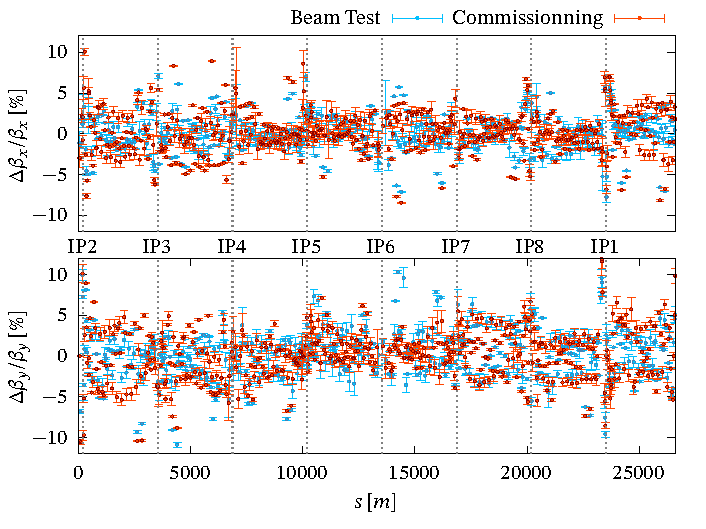
\includegraphics[width=0.49\linewidth]{images/beamtest/b1_bb.pdf}
    \hfill
    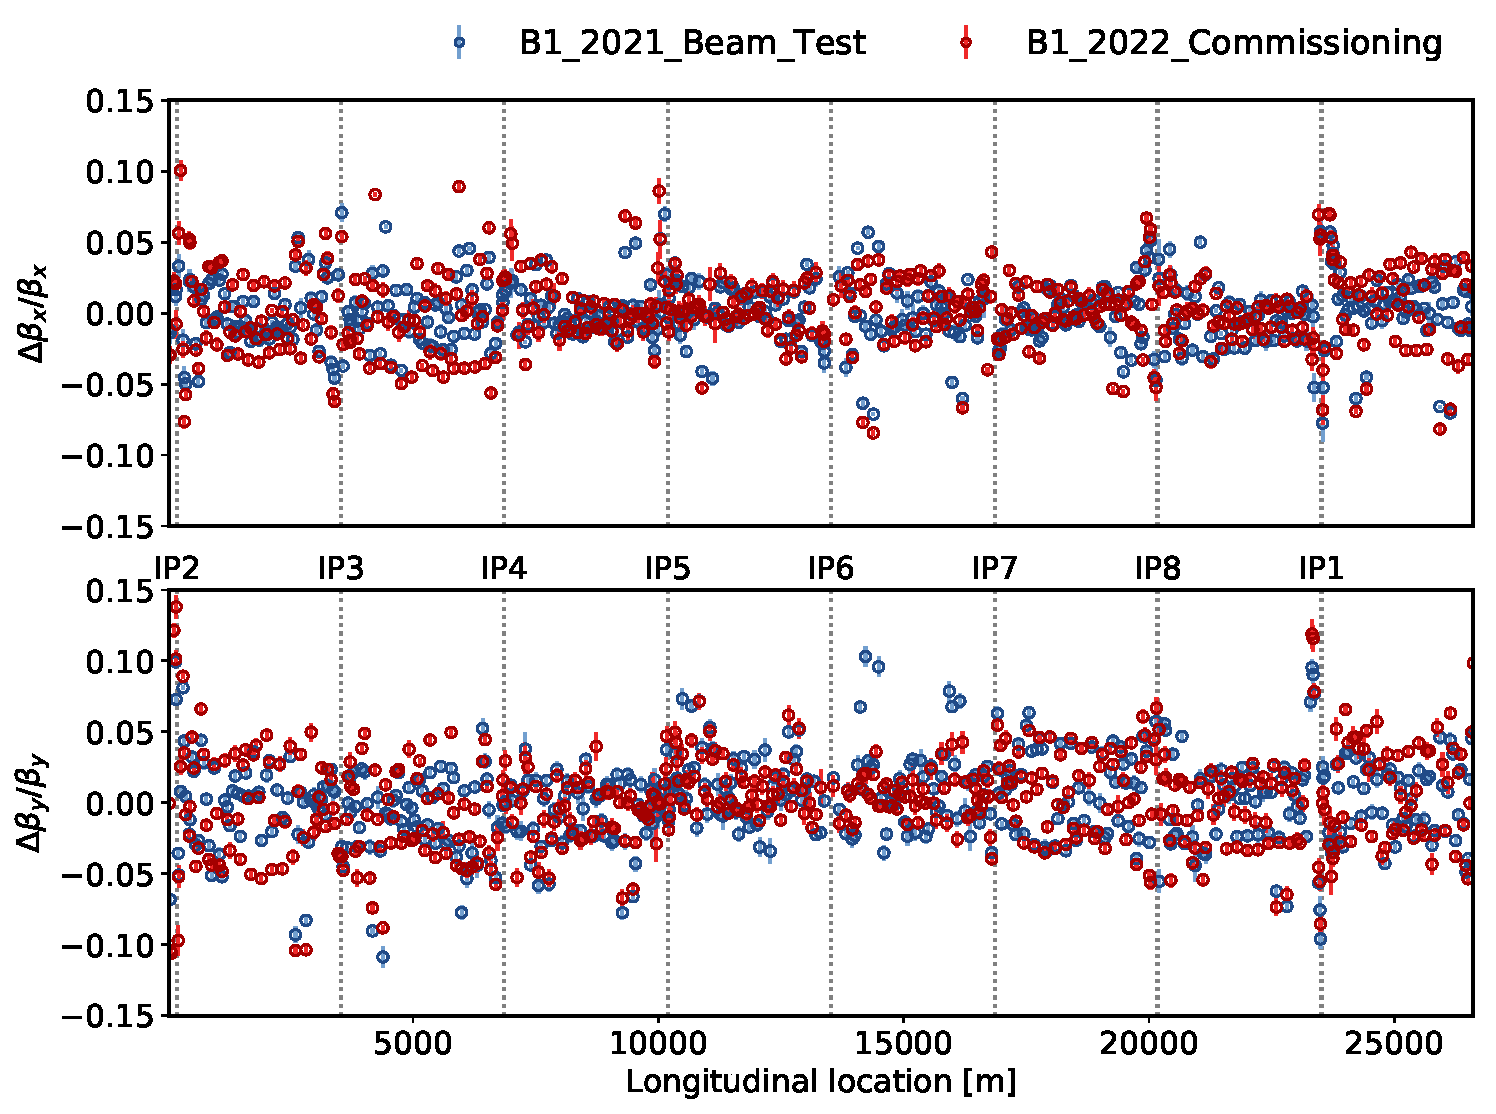
\includegraphics[width=0.49\linewidth]{images/beamtest/lhcb1_betabeat_vs_beamtest.pdf}
    
    Measured the injection optics with the corrections of \highl{2021 beam test}.
    Looks similar, \highl{no corrections} were re-calculated.
\end{frame}

\section{The Way to Top Energy}

\begin{frame}{Coupling in the Ramp}
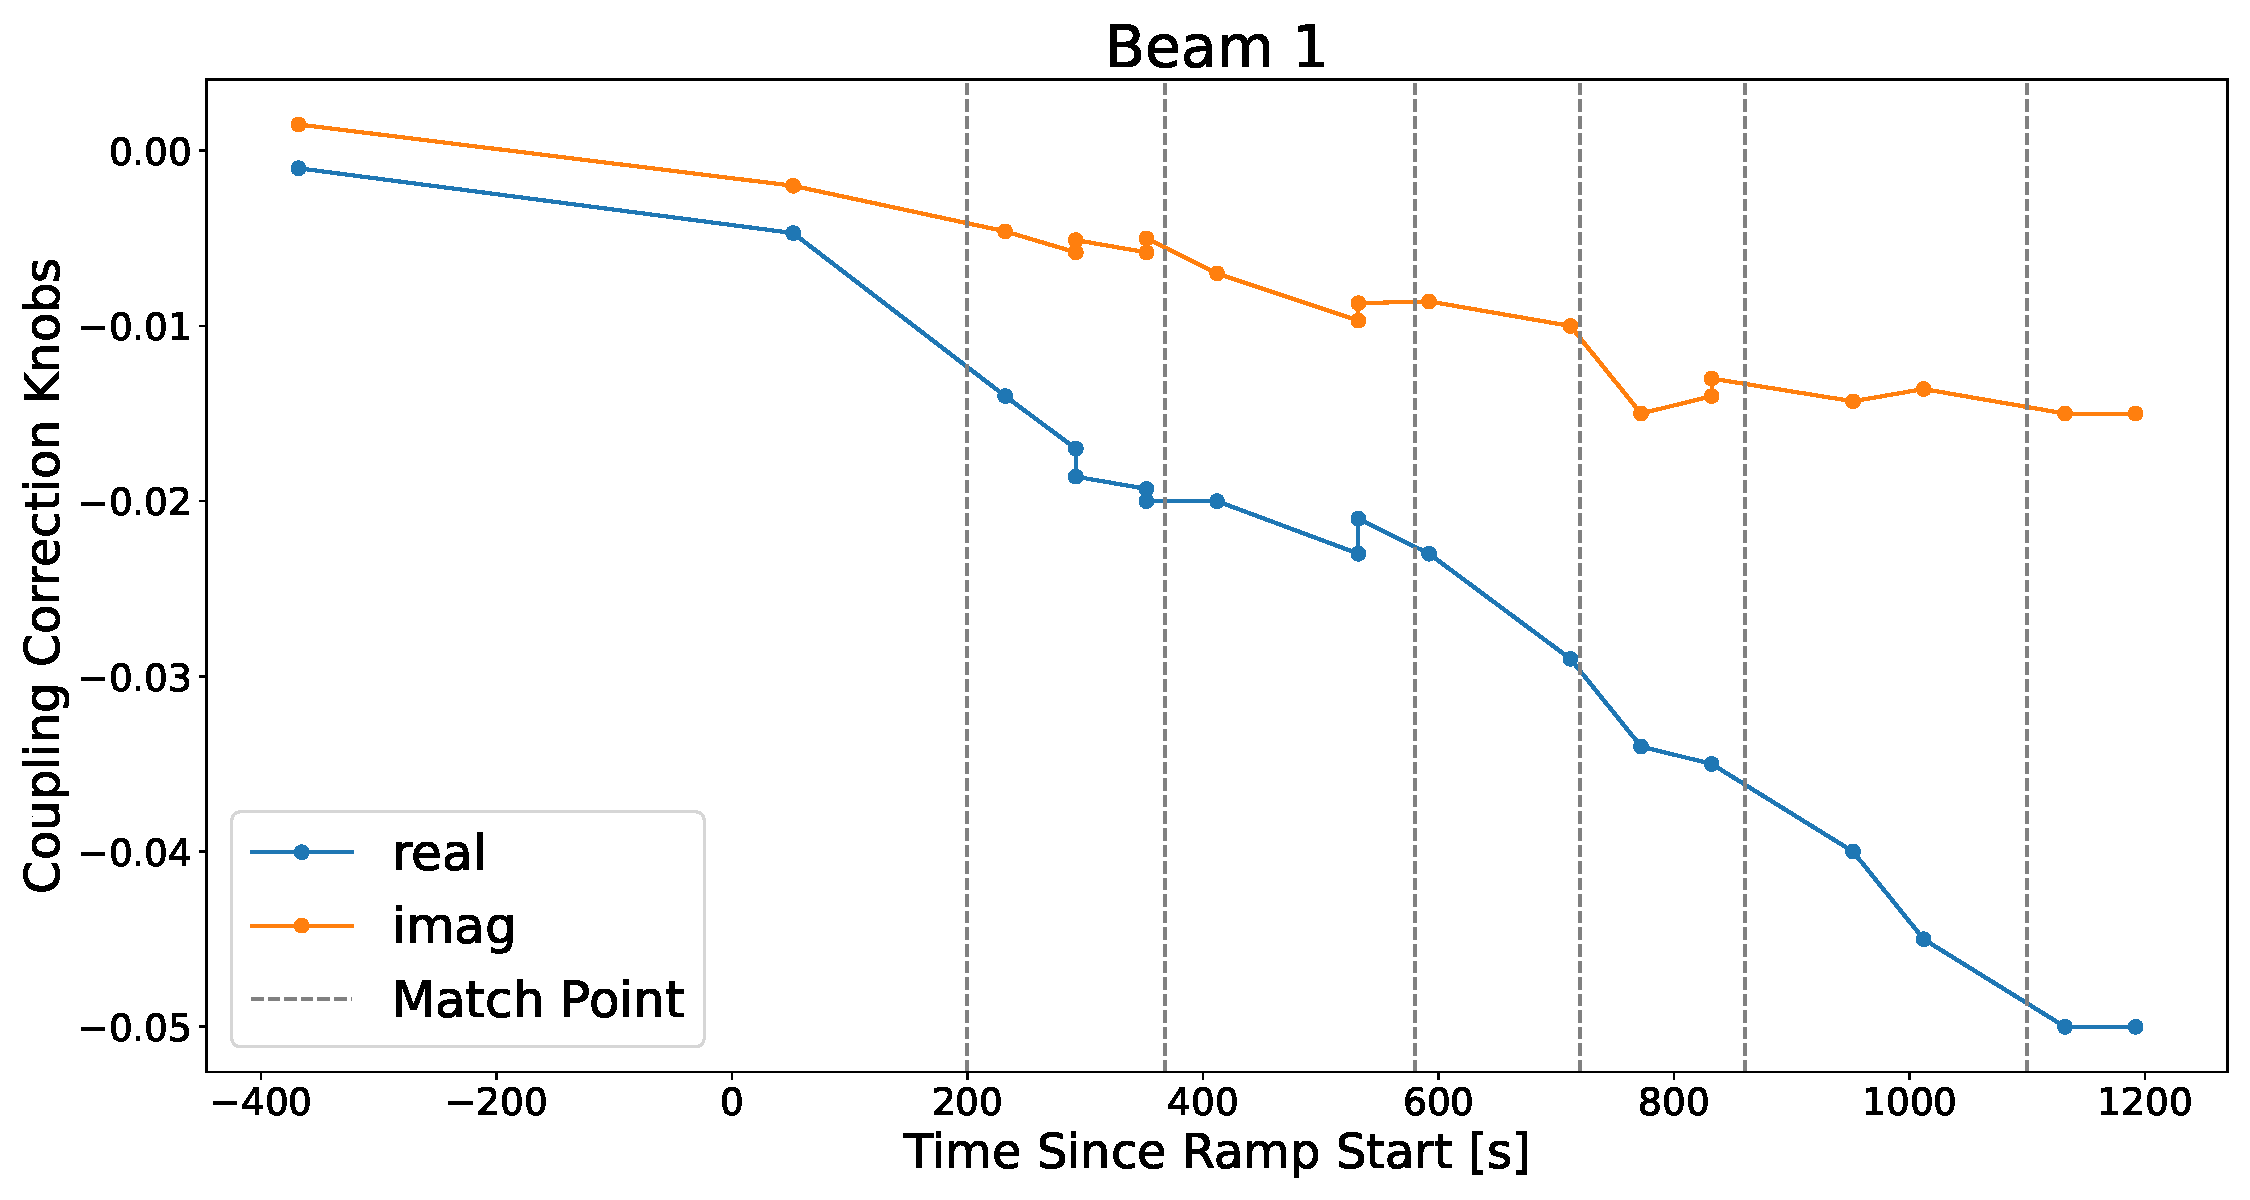
\includegraphics[width=0.49\linewidth]{images/ramp/B1_coupling_correction_knobs_in_ramp.pdf}
\hfill
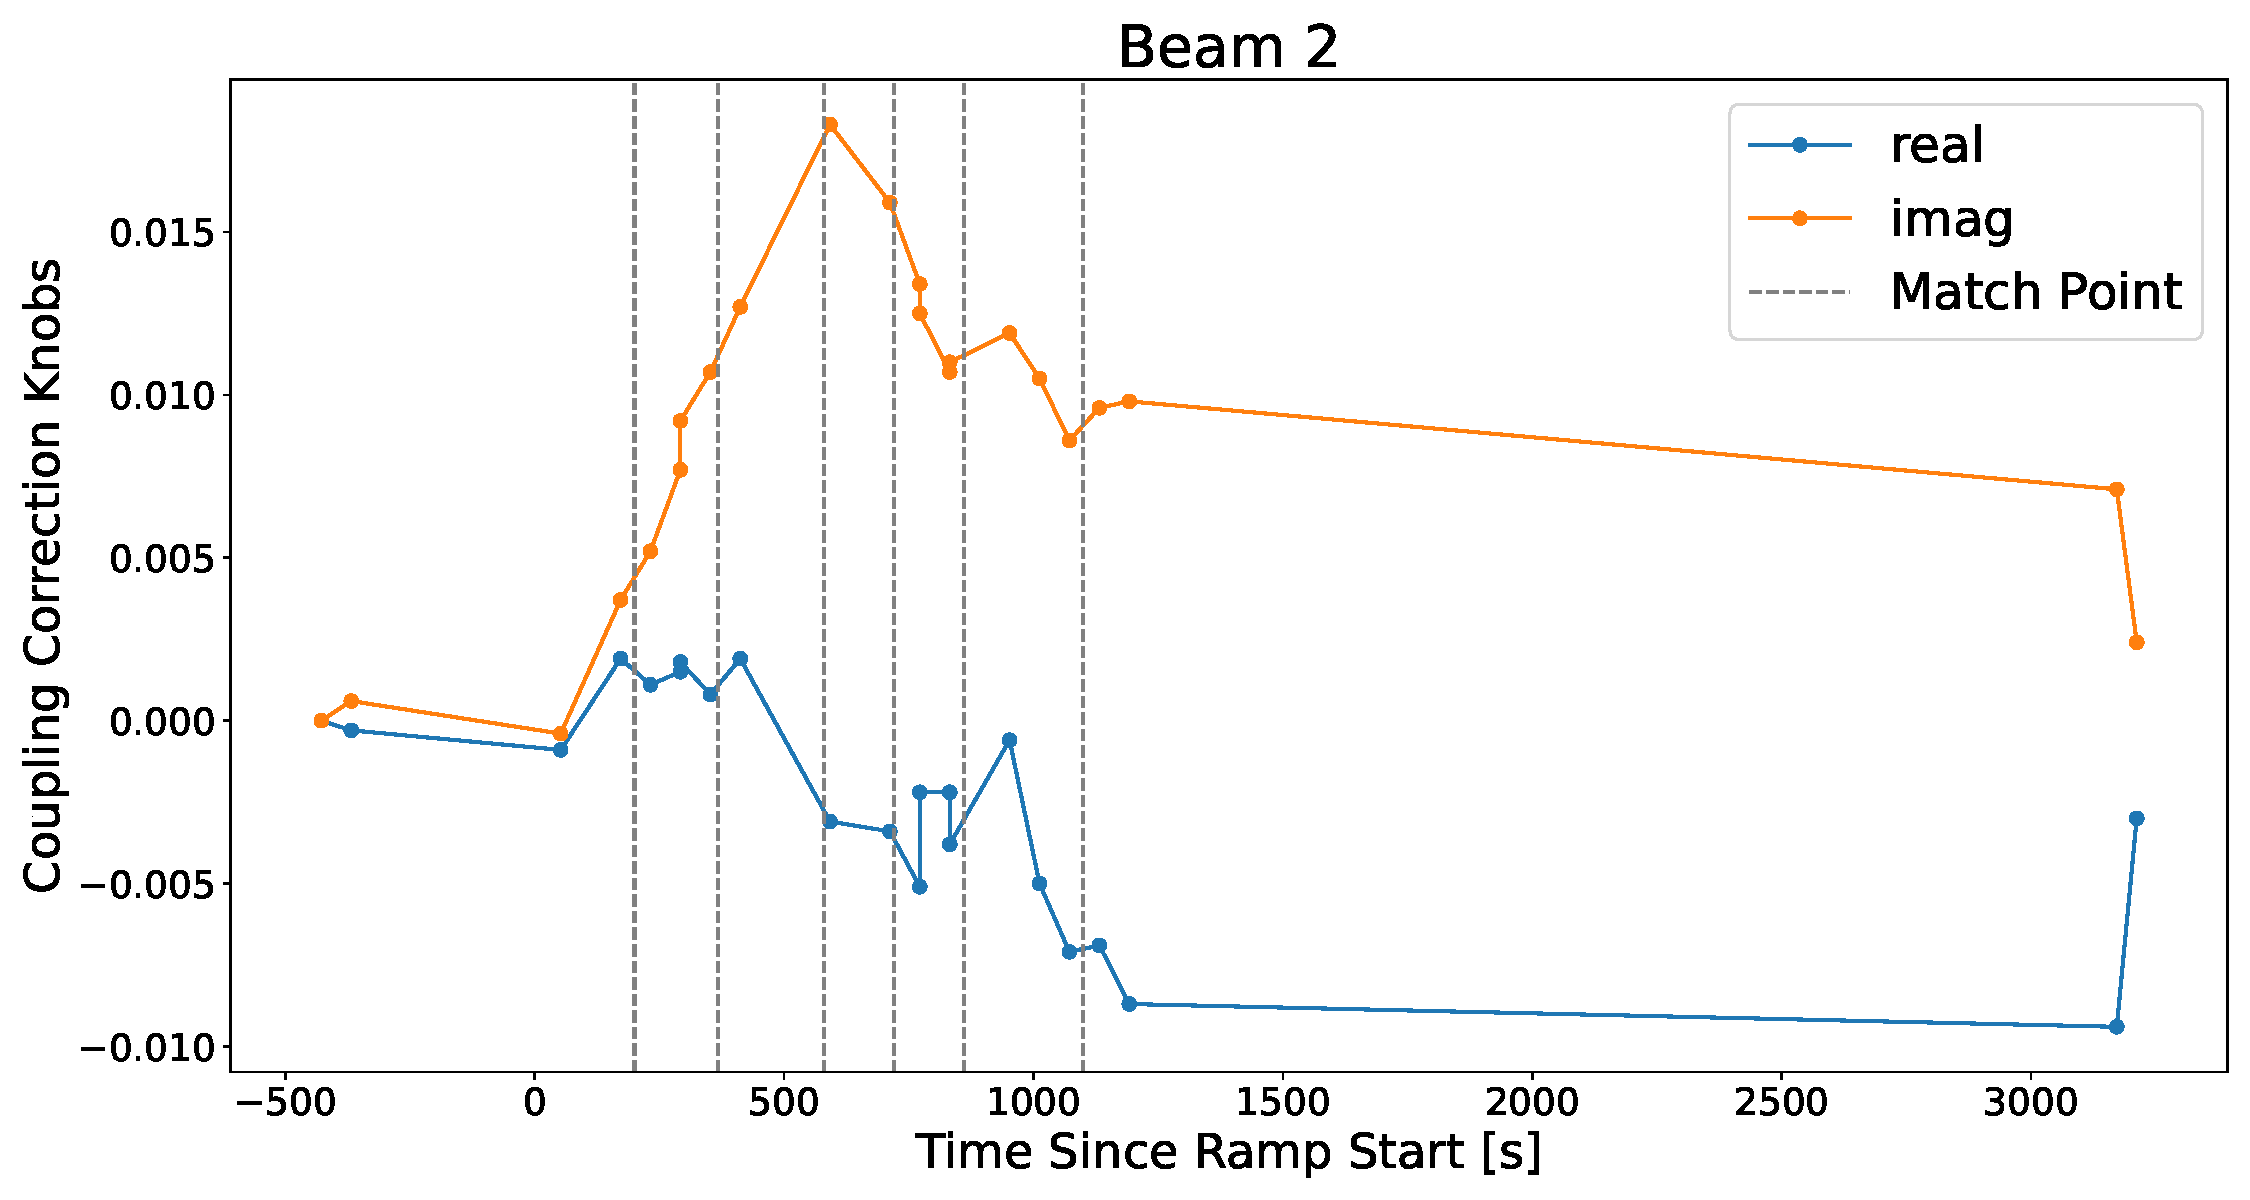
\includegraphics[width=0.49\linewidth]{images/ramp/B2_coupling_correction_knobs_in_ramp.pdf}

\begin{itemize}
    \item %
did \highl{manual coupling} measurement during the ramp because the coupling server
\highl{failed to give} good results 
    \item %
calculated \highl{coupling corrections} (verifying on the way that the selected model didn't deteriorate the calculations)
    \item %
these were \highl{programmed in} to be applied during the next ramp
    \item %
re-measure showed that we corrected \highl{$< 0.005$ at every pick-up point}
\end{itemize}
\end{frame}

\begin{frame}{6.8 TeV Optics}

\end{frame}

\section{Squeeze}

\begin{frame}{30cm Optics}
    
\end{frame}

% \backcover

\end{document}
